\section{Transfer and Meta-Learning}

% ---------------------------------------------------------------- Slide 2 (divider)
\begin{frame}{}
    \LARGE Transfer Learning and \textbf{Meta-Learning}
\end{frame}

% ---------------------------------------------------------------- Slide 3
\begin{frame}{What's the problem?}
\vfill
\begin{columns}[c]
\begin{column}{0.5\textwidth}
\centering
this is easy (mostly)\\[0.4em]
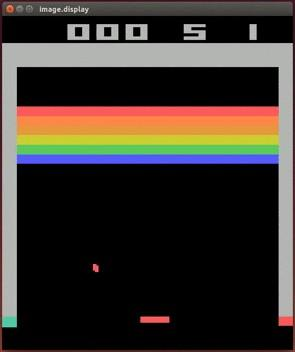
\includegraphics[width=0.5\linewidth]{images/meta-rl-open/figures/easy-atari.jpg}
\end{column}
\begin{column}{0.5\textwidth}
\centering
this is difficult\\[0.4em]
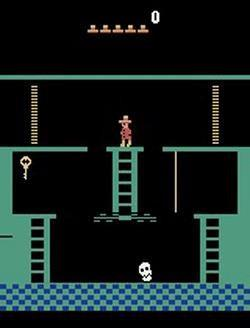
\includegraphics[width=0.5\linewidth]{images/meta-rl-open/figures/hard-real.jpg}
\end{column}
\end{columns}
\vfill
\begin{center}{\Large Why?}\end{center}
\vfill
\end{frame}

% ---------------------------------------------------------------- Slide 4
\begin{frame}[shrink=10]{Can RL use the same prior knowledge as us?}
\begin{center}
\raisebox{-0.5\height}{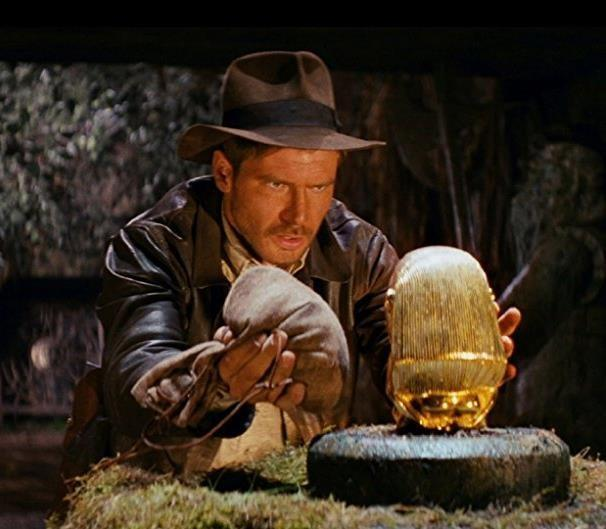
\includegraphics[height=1.9cm]{images/meta-rl-open/figures/s4-adventurer.jpg}}\qquad
\raisebox{-0.5\height}{
\includegraphics[height=1.0cm]{images/meta-rl-open/figures/s4-arrow.jpg}}\qquad
\raisebox{-0.5\height}{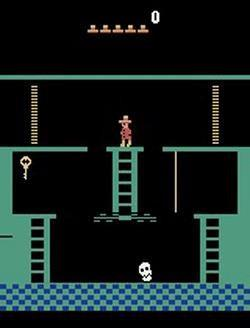
\includegraphics[height=2.1cm]{images/meta-rl-open/figures/s4-atari.jpg}}
\end{center}
\begin{itemize}
    \item If we've solved prior tasks, we might acquire useful knowledge for solving a
          new task
    \item How is the knowledge stored?
    \begin{itemize}
        \item \textbf{Q-function:} tells us which actions or states are good
        \item \textbf{Policy:} tells us which actions are potentially useful
        \begin{itemize}\item some actions are never useful!\end{itemize}
        \item \textbf{Models:} what are the laws of physics that govern the world?
        \item \textbf{Features/hidden states:} provide us with a good representation
        \begin{itemize}\item Don't underestimate this!\end{itemize}
    \end{itemize}
\end{itemize}
\end{frame}

% ---------------------------------------------------------------- Slide 5
\begin{frame}{How can we frame transfer learning problems?}
\begin{enumerate}
    \item \textbf{Forward transfer:} learn policies that transfer effectively
    \begin{enumerate}
        \item[a)] Train on source task, then run on target task (or finetune)
        \item[b)] Relies on the tasks being quite similar!
    \end{enumerate}
    \item \textbf{Multi-task transfer:} train on many tasks, transfer to a new task
    \begin{enumerate}
        \item[a)] Sharing representations and layers across tasks in multi-task learning
        \item[b)] New task needs to be similar to the distribution of training tasks
    \end{enumerate}
    \item \textbf{Meta-learning:} learn to learn on many tasks
    \begin{enumerate}
        \item[a)] Accounts for the fact that we'll be adapting to a new task during
                  training!
    \end{enumerate}
\end{enumerate}
\end{frame}

% ---------------------------------------------------------------- Slide 6
\begin{frame}{What issues are we likely to face?}
\begin{columns}[c]
\begin{column}{0.66\textwidth}
\begin{itemize}
    \setlength{\itemsep}{1.0em}
    \item \textbf{Domain shift:} representations learned in the source domain might not
          work well in the target domain
    \item \textbf{Difference in the MDP:} some things that are possible to do in the
          source domain are not possible to do in the target domain
    \item \textbf{Finetuning issues:} if pretraining \& finetuning, the finetuning
          process may still need to explore, but optimal policy during finetuning may
          be deterministic!
\end{itemize}
\end{column}
\begin{column}{0.34\textwidth}
\centering
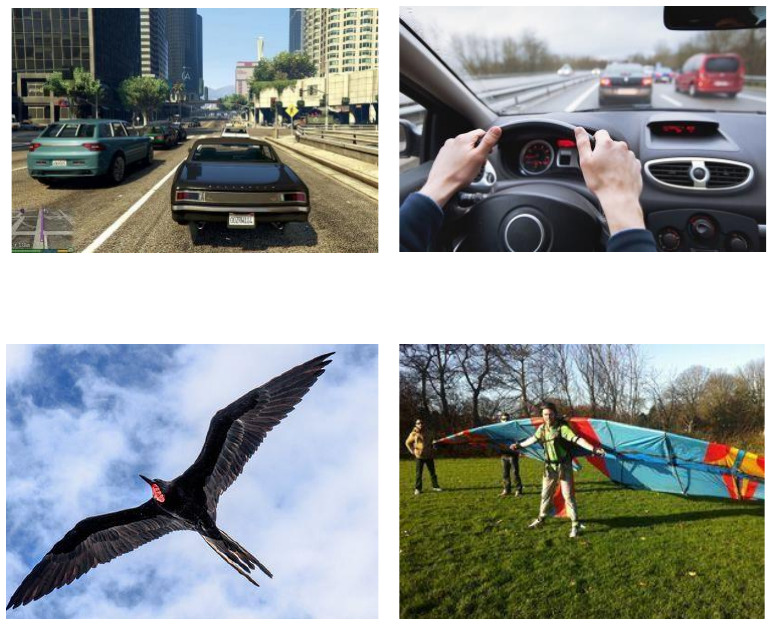
\includegraphics[width=\linewidth]{images/meta-rl-open/figures/s6-photos.jpg}
\end{column}
\end{columns}
\end{frame}

% ---------------------------------------------------------------- Slide 7
\begin{frame}{How can we frame transfer learning problems?}
\begin{enumerate}
    \item \textbf{Forward transfer:} learn policies that transfer effectively
    \begin{enumerate}
        \item[a)] Train on source task, then run on target task (or finetune)
        \item[b)] Relies on the tasks being quite similar!
    \end{enumerate}
    \item \textbf{Multi-task transfer:} train on many tasks, transfer to a new task
    \begin{enumerate}
        \item[a)] Sharing representations and layers across tasks in multi-task learning
        \item[b)] New task needs to be similar to the distribution of training tasks
    \end{enumerate}
    \item \textbf{Meta-learning:} learn to learn on many tasks
    \begin{enumerate}
        \item[a)] Accounts for the fact that we'll be adapting to a new task during
                  training!
    \end{enumerate}
\end{enumerate}
\end{frame}
